\chapter{評価}
\label{chap:evaluation}

本章では、前章で提案した手法で実装したアルゴリズムのAIを\ref{chap:implementation}章で実装した1人麻雀で打たせ、和了率を評価する。
1人麻雀では和了率についてのみ評価した。また、人間プレイヤーとの比較、アルゴリズム同士の比較をそれぞれ別の対戦数で行った。
同様に4人麻雀で打った際の成績も評価する。4人麻雀の評価項目は、和了率、放銃率、レーティングである。

\section{1人麻雀における成績の評価}
提案手法で提示した、期待和了順目の評価による打牌選択のアルゴリズムを1人麻雀に適用し、性能を評価した。なお、実装環境は前章で示した表\ref{imp2}と同じである。
図\ref{100houra}に示すのは、同じ5000局のテストデータを与え、対局を行うごとに和了率を測定し更新していったときのグラフである。横軸を対局数、縦軸を和了率とした。対局数が50戦以下の場合では、極端に母数が少なく和了率の分散が大きいため、グラフに示すのは50戦以上の対局の結果とした。

図\ref{100houra}に示すアルゴリズムの詳細について述べる。

\begin{itemize}
 \item {\bf シャンテン数} \mbox{}\\ 
  選択した打牌が元の牌姿に比べて、シャンテン数が最も少なくなるような牌を選択して打牌するアルゴリズムである。
  そのような牌が複数存在する場合はその中からランダムに決定し、打牌する。
 \item {\bf 有効牌} \mbox{}\\
      上記の「シャンテン数」のアルゴリズムの中で、複数の牌が存在するときに更に優劣を比較して打牌を決定するアルゴリズムである。
      シャンテン数を下げる牌の集合の中から、それぞれを切った場合の有効牌の枚数を比較して最も多いもの選択肢、打牌する。
 \item {\bf 期待和了巡目} \mbox{}\\
      本研究で提案した、打牌した時にその手の期待和了巡目が最も小さいものを選択するアルゴリズムである。
      期待和了巡目とは与えられた牌姿が和了までにかかる平均消費巡目を指すもので、本論文においての詳細な定義は\ref{chap:approach}章によるものとする。
\end{itemize}

\begin{figure}[H]
 \centering
 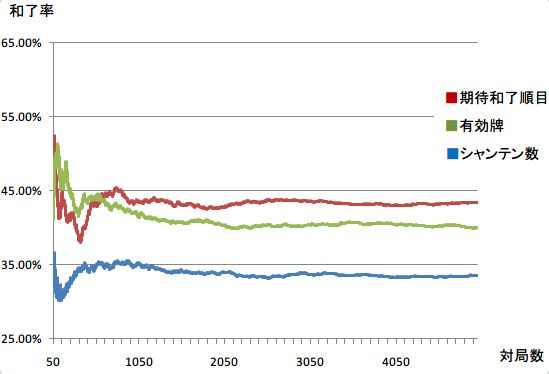
\includegraphics[keepaspectratio, scale=0.8,bb=0 0 549 374]
      {img/1houra.jpg}
 \caption{1人麻雀の和了率遷移}
 \label{1houra}
\end{figure}


始めの約500戦では、どのアルゴリズムも概ね下降をし続けた。これは、この付近の対局で使われたデータセットが元々和了しにくいものであったと考えられる。例えば、シャンテン数が元々大きい集合体が偏ることで、どのアルゴリズムであっても27回のツモまでに和了出来ないケースが多くなるからである。しかし、全体として下降している傾向があるものの、同じデータセットを使っている中で「シャンテン数」のアルゴリズムは他のアルゴリズムに比べて和了率が明らかに低い。このことから、約500戦であってもある程度「シャンテン数」のアルゴリズムは和了率の観点からは劣ると考えられる。また、他の2つのアルゴリズムである「有効牌」と「期待和了巡目」については、約500戦の結果では和了率の差が明確ではない。したがって更に対局数を増やした結果を見る必要がある。

対局数が1000戦を超えると、どのアルゴリズムもほぼ横ばいの和了率になっていった。そして5000戦到達した時には、それぞれのアルゴリズムの和了率には明確な差が見られた。最終的な和了率は「シャンテン数」が33.58%、「有効牌」が40.10%、「期待和了巡目」が43.42%となった。

次に、天鳳において実力が上位0.1%に当たる上級者(本論文執筆者)と、天鳳において全体の50%に当たる平均プレイヤーを一人ずつ用意し、100局のテストデータで同じく和了率を比較した。その結果を表\ref{1houra}に示す。この場合も同じテストデータで他のアルゴリズムによる和了率も測定している。また、表\ref{1houra}に示すそれぞれのアルゴリズムについては、詳細は図\ref{1houra}においてのものと同じである。




\begin{table}[h]
  \caption{100局のデータセットでの和了率}
  \label{100houra}
  \begin{center}
  \begin{tabular}{c|c}
    \hline
    プレイヤー   & 和了率(\%)\\\hline\hline
    上級者 	& 53 \\\hline
    期待和了巡目 & 44 \\\hline
    有効牌 	& 41 \\\hline
    平均プレイヤー 	& 36\\\hline
    シャンテン数	& 32 \\\hline
  \end{tabular}\end{center}
\end{table}

1人麻雀を5000局打たせたことによる和了率の比較では、「シャンテン数」<「有効牌」<「期待和了巡目」という結果となった。これは統計的に優位な水準での優劣である。結果については期待通りで、シャンテン数を下げるだけのアルゴリズムに対し、それをさらに有効牌の数を比べるアルゴリズムでは和了率が上昇した。また、本研究で提案した「期待和了巡目」のアルゴリズムでは、さらに有効牌の中でもより和了までの到達度を正確に計算することで和了率が上がることが確認された。1人麻雀による対局では、多人数性が存在しないため、本手法がうまく適用できると考えられる。また、上級者と平均実力者の人間プレイヤーを加えた100局の対局では、期待和了巡目のアルゴリズムの和了率は平均プレイヤーより優り、上級者に劣る結果となった。これは、上級者の場合はシャンテン数が瞬間的にあえて最小でないような打牌をして結果的に和了率がもっとも高くなる場合が存在するからであると考えられる。期待和了巡目はシャンテン数が最小になる牌の中から打牌を選択しているため、このような選択が行えない。
% \subsection{期待平均和了順目の探索の深さの評価}
% \subsection{モンテカルロ法の探索領域}


\section{4人麻雀における成績の評価} %麻雀サーバーとの対戦
本研究では1人麻雀における和了率の上昇を目指すため、静的指数である期待和了巡目を利用し、打牌を決定するアルゴリズムを提案した。これを第4章で設計した実装を元に、オンライン麻雀天鳳で打たせ、その成績を集計した。なお、実装環境は前章で示した、表\ref{imp1}と同じである。
対戦した場所は天鳳の一般卓で、ルールは喰いアリ赤アリの東風戦、持ち時間は3秒である。2016年11月から2017年1月までの期間対戦を行い、試合数は2231戦となった。同じように、関連研究では1人麻雀のアルゴリズムを4人麻雀に適用し、実際の対人戦でその成績を評価している例が存在する。この節では、それらの研究の成績と本手法の比較を行い、その優位性を評価した。

評価として、和了率、放銃率、レーティングを比較した。


\subsection{和了率}
4人麻雀で実装した自動打ちシステムを対戦させた結果の、和了率の遷移を図\ref{houra2231}に示す。横軸を対局数、縦軸を和了率とした。
50戦以下の対局では母数が少ないために和了率の分散が大きいため、図は50戦以上の対局からの和了率を掲載した。和了率は300戦までは分散が大きかったが、500戦を超えると徐々に収束していき、2231戦後の最終和了率は21.290%となった。

\begin{figure}[h]
 \centering
 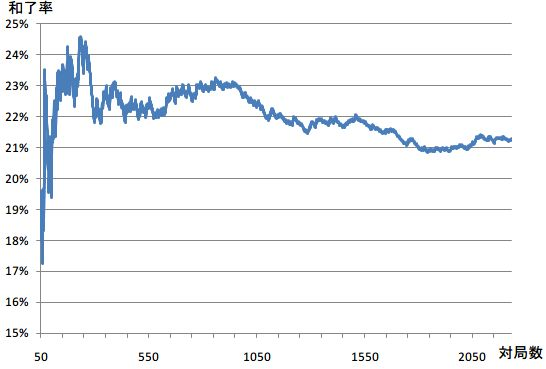
\includegraphics[keepaspectratio, scale=0.8,bb=0 0 546 369]
      {img/houra2231.jpg}
 \caption{和了率遷移}
 \label{houra2231}
\end{figure}

また、関連研究と比べた結果の表\ref{tb:houraritu}に示す。
佐藤らは有効牌を数え上げることによって打牌を選択するアルゴリズムを使用したが、その中で再帰の深さを変えたりヒューリスティックを加えたり複数の手法においてのデータを取っている。ただしそれらによる差は統計的に優位なほど大きな差ではなかったため、今回はそれらの中で最も基本的である再帰の深さ1のものと比較した。また、表にある平均プレイヤーとは、天鳳において平均レートが1500付近である初段のプレイヤーとした。そのデータは天鳳\cite{tenhou}のランキングページに公開されているものを引用した。

\begin{table}[h]
  \caption{4人麻雀においての和了率の比較}
  \label{tb:houraritu}
  \begin{center}
  \begin{tabular}{c||c|c|c|c}
    \hline
    プレイヤー   & 本研究 & 佐藤らの研究 & 水上らの研究 & 平均プレイヤー\\\hline\hline
    対局数   & 2231 & 2526 & 504 & -\\\hline
    和了率(\%) & 21.3 & 20.1 & 18.8 & 21.9\\\hline
  \end{tabular}\end{center}
\end{table}

和了率を比較すると、本手法は佐藤らの研究をわずかに上回る結果となった。佐藤らの研究では有効牌の数え上げによって打牌を選択しているが、本手法では平均和了巡目を用いることでより先の展開を考慮した打牌の選択が可能になっていると考えられる。これは事前に期待されていたとおりであった。しかし、大きな差が生まれたというわけではなく、平均プレイヤーを優位に超えることはできなかった。


\subsection{放銃率}
次に、放銃率の遷移を図\ref{houzyu2231}に示す。横軸を対局数、縦軸を放銃率とした。
50戦以下の対局では母数が少ないために放銃率の分散が大きいため、図は50戦以上の対局からの放銃率を掲載した。放銃率は500戦までは下降を続けたが、1000戦を超えると徐々に収束していき、2231戦後の最終放銃率は18.377%となった。
\begin{figure}[h]
 \centering
 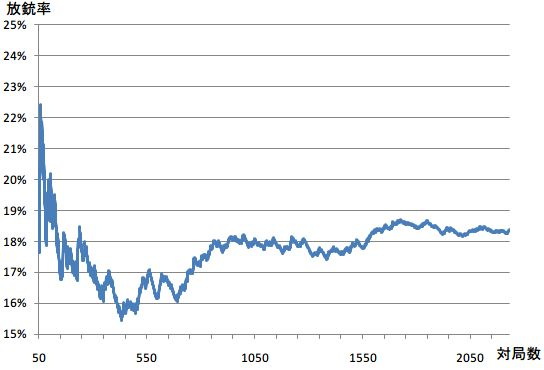
\includegraphics[keepaspectratio, scale=0.8,bb=0 0 544 370]
      {img/houzyu2231.jpg}
 \caption{放銃率遷移}
 \label{houzyu2231}
\end{figure}

また、関連研究と比べた結果を表\ref{tb:houzyu2231}に示す。
放銃率においてはどの研究にも大きな差は見られなかった。これらの研究では、4人麻雀におけるオリの戦略を加えていないからであると考えられる。平均プレイヤーはオリを行っているため、放銃率が低い。4人麻雀においては放銃率による失点は成績を悪くするため、重要な指標であるが、これらはオリの戦略を実装することで改善する必要があると考えられる。

\begin{table}[h]
  \caption{4人麻雀においての放銃率の比較}
  \label{tb:houzyu2231}
  \begin{center}
  \begin{tabular}{c||c|c|c|c}
    \hline
    プレイヤー   & 本研究 & 佐藤らの研究 & 水上らの研究 & 平均プレイヤー\\\hline\hline
    対局数   & 2231 & 2526 & 504 & - \\\hline
    放銃率(\%) & 18.4 & 18.9 & 19.0 & 16.4\\\hline
  \end{tabular}\end{center}
\end{table}

\subsection{レーティング}
レーティングとは、特定のプレイヤーが他のプレイヤーと比較してどの程度成績が良いかを図る評価の仕方の一つである。
レーティングは、平均順位と負の相関を持ち、式\ref{rate}で計算される。ゲームを行ったときの卓の平均のレーティングを$R_{ave}$とし、ゲームの結果の順位を$Rank$、ゲームを行う前のレーティングを$R$とした時、そのゲームによって更新されるレーティングがR'である。初期の時点でのレーティング($R$)は1500である。
\begin{equation}
\label{rate}
\Large R' = R + (50 - Rank × 20 + \displaystyle \frac{R_{ave} - R}{40} ) × 0.2
\end{equation}

4人麻雀で実装した自動打ちシステムを対戦させた結果の、レーティングの遷移を図\ref{rate2231}に示す。横軸を対局数、縦軸をレーティングとした。
50戦以下の対局では母数が少ないためにレーティングの分散が大きいため、図は50戦以上の対局からのレーティングを掲載した。レーティングは500戦までは分散が大きかったが、1000戦を超えると徐々に収束していき、2231戦後の最終レーティングは1382となった。

\begin{figure}[h]
 \centering
 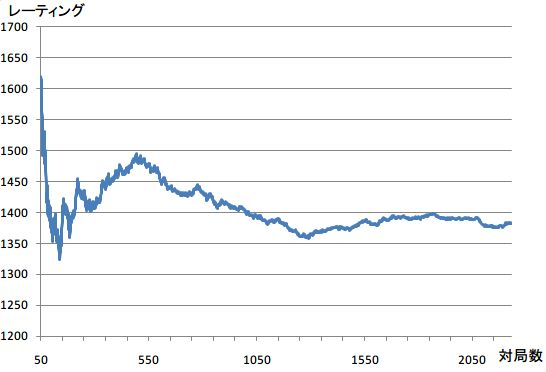
\includegraphics[keepaspectratio, scale=0.8,bb=0 0 546 372]
      {img/rate2231.jpg}
 \caption{レーティング遷移}
 \label{rate2231}
\end{figure}

また、関連研究と比べた結果を表\ref{tb:rate2231}に示す。
レーティングは佐藤らの研究をわずかに上回るという結果になった。しかし大きな有意差は見られず、平均プレイヤーにも及ばなかった。これは和了率の観点では本研究が優位なものの、四人麻雀では多人数性の理由によりほかの影響が多いことが考えられる。理由としては、1人麻雀では和了率が本研究の方が高いものの、放銃率では平均プレイヤーが低く出ているため、オリの影響が大きいと思われるからである。

\begin{table}[h]
  \caption{4人麻雀においてのレーティングの比較}
  \label{tb:rate2231}
  \begin{center}
  \begin{tabular}{c||c|c|c}
    \hline
    プレイヤー   & 本研究 & 佐藤らの研究 & 平均プレイヤー\\\hline\hline
    対局数   & 2231 & 2526 & - \\\hline
    レート & 1382 & 1339 & 1558\\\hline
  \end{tabular}\end{center}
\end{table}

\section{考察}

以上で示した評価において、1人麻雀と4人麻雀のそれぞれの和了率を表\ref{4houra}にまとめる。ここでの1人麻雀の和了率は表\ref{100houra}に示した値、4人麻雀の和了率は表\ref{tb:houraritu}の値を用いた。4人麻雀においての有効牌アルゴリズムの値は、佐藤らのものを引用している。

\begin{table}[h]
  \caption{4人麻雀においての和了率の比較}
  \label{4houra}
  \begin{center}
  \begin{tabular}{c||c|c|c|c}
    \hline
    プレイヤー  & 期待和了巡目 & 有効牌 & 平均プレイヤー & 上級者\\\hline\hline
    1人麻雀の和了率(\%) & 44 & 41 & 36 & 53\\\hline
    4人麻雀の和了率(\%) & 21.3 & 20.1 & 21.9 & 27.3\\\hline
  \end{tabular}\end{center}
\end{table}

1人麻雀の和了率は、期待和了巡目のアルゴリズムが平均プレイヤーと有効牌のアルゴリズムを抑え高い数値を出している。これは、期待通り期待和了巡目のアルゴリズムが1人麻雀にうまく適用できたと考えられる。しかし、上級者には及ばず、これ以上和了率を上げるためにはさらなるアルゴリズムの改善が必要である。本研究の提案する、期待和了巡目を用いた打牌アルゴリズムでは、有効牌を更にブロックごとに分けることで、有効牌を単に数だけで比較するのではなく期待和了巡目という観点から比較している。この結果、単に有効牌の数だけを比較するアルゴリズムよりも高い和了率を出すことが出来たが、今回の期待和了巡目では複雑になると思われる部分を一部仮定による概算で求めている。例えば、それぞれのブロックをツモる確率は手の進み方により一定と仮定している。実際には手の進みによって変化する場合があるので、それを考慮したモデルを作ることで、さらなる和了率の上昇が期待できる。

4人麻雀の和了率は、期待和了巡目のアルゴリズムが有効牌のアルゴリズムよりわずかに高い数値を示したものの、平均プレイヤーを超えることは出来ないという結果になった。表\ref{4houra}の1人麻雀の和了率と4人麻雀の和了率を比較してみると、1人麻雀による和了率は平均プレイヤーを明らかに超えているが、4人麻雀では大差がない。このことから、4人麻雀における和了率は多人数性による影響が強く影響していると考えられる。4人麻雀の和了率に影響を与える要素としては、鳴きによる和了や相手プレイヤーの和了による終局などが考えられる。鳴きを研究したアルゴリズムでは平均プレイヤーの和了率を超えたという報告もされており\cite{mizukami},鳴きによる研究は特に重要だと考えられる。



% このように、レートは本手法の方が上回る結果となった。ここで保証安定レートについて比較をする。



